\chapter{System Evaluation}\label{chap:eval}
One of the aims stated for this study, as listed in the Chapter~\ref{sec:Introduction}, was to write a Python application with scalability in mind. Therefore, this chapter is devoted to presenting a thousand-feet view of the application so that the implementation described in former chapters could be taken as only one of the many possibilities to realise the intended system characteristics as well as functionality. The second section of the chapter presents a discussion of SmartNotes application metrics gathered using benchmarking tools such as \texttt{httperf}~\cite{httperf_tool} or \texttt{autobench}~\cite{autobench_tool} and statistics from the Google App Engine dashboard. The present chapter, together with Chaper~\ref{cha:conclusions}, also summarises the results of the subject of this study.
 
\section{Presentation of the final result}\label{sec:result}
Apart from a client-server architecture whose segments were presented in Figure~\ref{fig:smartnotes_components}, SmartNotes has the features of flexibility, scalability and security described in Section~\ref{sec:gae}. The web interface of the application is a simple, internationalized one that provides general information about the project and allows the iterated users access its functionality. Currently, the latter involves merely creating a SmatNotes account by using the Google Account as described in Section~\ref{subsec:ismartnotes_activation} and later receiving an activation key, the process being straightforward as presented in Figure~\ref{fig:sn_web_interface}. Finally, the users pass the activation code to the iSmartNotes application in order to take the advantage of synchronization feature allowing the users, as described in Section~\ref{sec:functionality_descr}, to work on their notes and perform synchronization whenever they may wish. The main iSmartNotes window is presented in Figure~\ref{fig:ismartnotes_window}; specifically, it has a simple text area where notes can be edited, and a \texttt{Sync} button that, depending on network connectivity, will perform synchronization on the local machine or additionally using the SmartNotes network infrastructure. This basic attempt realises the functionality, excluding sharing and grouping notes which are extensions to the present functionality and will be added to the SmartNotes application beyond the focus and implementation completed in this study. It can be clearly noted that the tool cannot compete with such applications like the ones introduced in Section~\ref{sec:popular_apps}. Yet, the related work was used as a inspiration for creating a scalable foundation that could be later become more complex by adding additional functionality, hence making the gathered experience further expanded and rendering SmartNotes more attractive to users. Finally, the SmartNotes blog, feedback form and hosting the source code on a well known Open Source service does not only point to gather users’ attention, but also to find developers who find the idea interesting and collaborate on it.
 
Technologies chosen here provide a well documented and truly active environment with a relatively low access barrier allowing direct involvement in a short time. Some of the chosen solutions, like Django or Mercurial, could become substituted with their equivalents among different language environments or using the Java language as a universal binding for the tools\footnote{Java programming language is wide know for its dynamic curve of development and impressing thread management. These features are few on the list of characteristics motivating the existence of such projects as JRuby, Jython or Quercus which are Java implementations of respectively Ruby, Python and PHP languages. That way, different runtimes can be used in one common environment, taking advantage of all of Java’s features.}.      
\begin{figure}[ht]
  \begin{center}
    \subfigure[\textbf{SmartNotes homepage with basic information and authentication}.]{\label{fig:sm_main}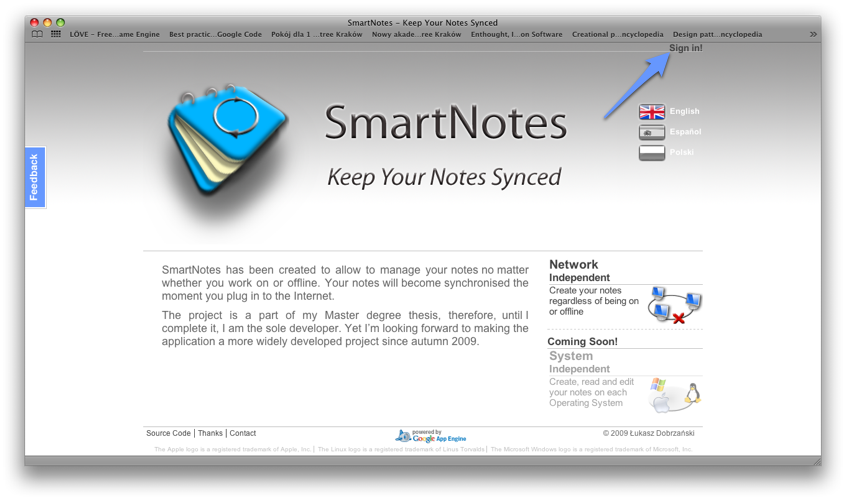
\includegraphics[scale=0.5]{img/SNmain_page.png}}
    \subfigure[\textbf{Authentication using the Google account}.]{\label{fig:sm_signin}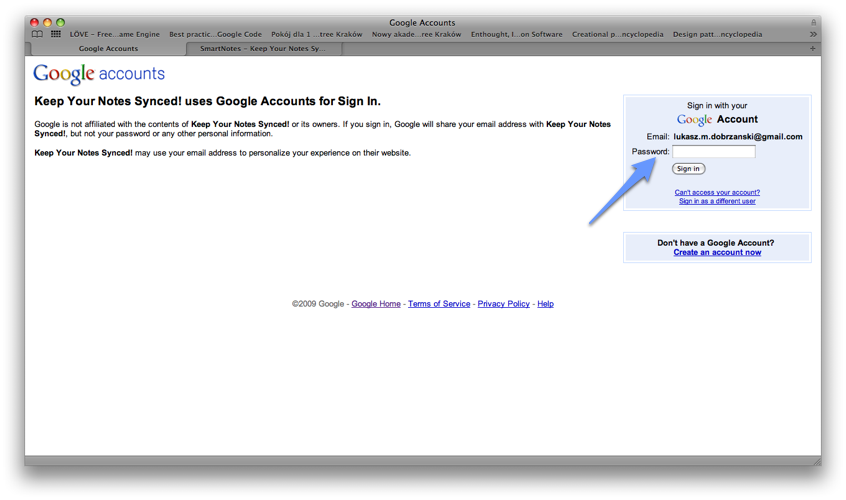
\includegraphics[scale=0.24]{img/SN_signin.png}}
    \subfigure[\textbf{Obtaining the SmartNotes activation key}.]{\label{fig:sm_getSNkey}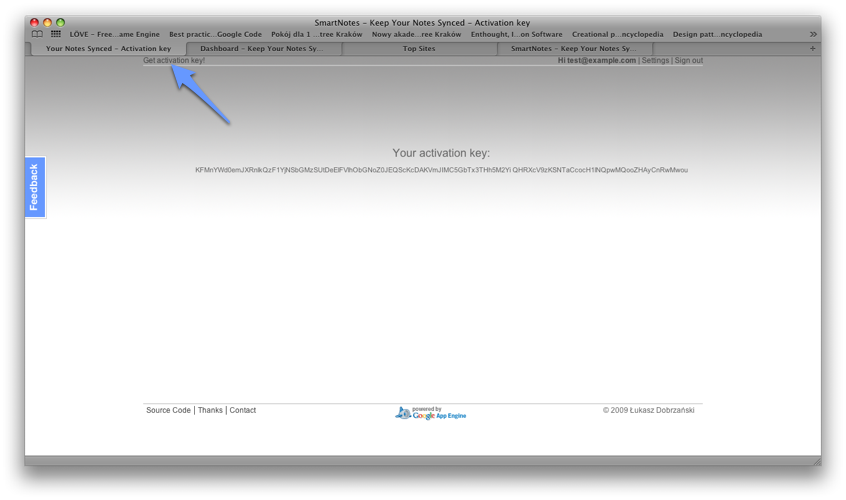
\includegraphics[scale=0.24]{img/SNget_activation_key.png}}
  \end{center}
  \caption{The view on the public web-based SmartNotes interface with basic information regarding the project and authentication.}
  \label{fig:sn_web_interface}
\end{figure}
That direction of development appears to be gathering popularity and is worth attention. \\However, the chosen set of components has proofed it value. This includes:
 \begin{itemize}
        \item{Google App Engine -- as a platform providing scalable infrastructure and additional useful API's for mailing, imaging or remote task queues.}
        \item{Django famework -- one of Python web frameworks which attracts more and more developers trough its clean architecture, out-of-the-box usability and strong community.}
        \item{Mercurial -- pure Python version control system with a well-designed support for HTTP protocol and a zero cost of administration.}
 \end{itemize}
It allowed to carry out the desired functionality with easiness for further development, an aspect that should be always recalled during any design process or when choosing between concurrent solutions. That, combined with system streamlining for concrete use cases, determines why the entire system concept is highly desirable when building scalable systems.
        
\begin{figure}[ht]
\begin{center}
\includegraphics[scale=0.5]{img/SN_ismartnotes_window.pdf}
\caption{The view on the iSmartNotes application window.}
\label{fig:ismartnotes_window}
\end{center}
\end{figure}
 
\section{Performance tests}\label{sec:performance}
The form of performance testing strongly depends on the scope of research. \texttt{Testing the application performance} is more a general name for the process that requires to become narrowed to a single parameter or a set of well defined properties. The usage of the right tool also matters to the same extent as making appropriate assumptions and choosing the right model to use – otherwise, measured values could not match the real application characteristics.  
 
The analyses done in this chapter follow the guidelines as defined in~\cite{gae_best_practises_plus_load_tests}, for testing applications using Google App Engine:
\begin{itemize}
              \item{Use production system. Most of web frameworks provide certain development environment including a server that can easily run on the local machine. What increases the speed of the development lifecycle at one side cannot be used for production purposes as this environment differs significantly from the deployment system and fails to produce much absolute measures about the final system performance.}
              \item{Gradual ramp up. The goal of load tests is to probe system reactions for certain sets of input parameters. Therefore, it is strongly desirable to make the probing resemble realistic cases. Besides, the resources of Google App Engine are granted only when the application demands them, which motivates a wrap-up round just before the actual test takes place.}
              \item{Realistic load. Is seems pointless to run tests for a situation that the system is unlikely to reach.}
\end{itemize}
The following part of this subsection presents a graphical illustration of selected performance metrics of the SmartNotes application running on Google App Engine. Taking into account parameters such as the rate of opened connections and reached request rate, the analysis will firstly focus on the variations of the response rate and will be finalized with a comparison of the average response time between different techniques, the latter including an internalized dynamic content, cached page and same page served as static content. The first is the most classical case when certain parts of page are determined by the state of the system; the second one makes use of a highly popular caching technique, whereas the last one utilizes special infrastructure devoted only to serving static content. All of these will be discussed more widely in relation to the obtained results.
 
The view on the dashboard of the SmartNotes application shown in Figure~\ref{fig:sn_dash_view} exposes a plot of request rate timeline for two different scenarios. The first one, marked as~\textit{(a)}, illustrates a regular usage case with no special anomalies, whereas the second figure~\textit{(b)} presents a case when outgoing bandwidth beccomes exceeded. This is the most basic way of tracking the application performance and status. Providing a couple of other tools which were discussed in Section~\ref{sec:gae_general}, admin interface is truly functional as well as easy to use. Providing a log browser, additionally, leaves a place where developers can put application-specific information on several logging levels.    
\begin{figure}[ht]
  \begin{center}
    \subfigure[\textbf{Regular situation with the average of about one\newline request per second}.]{\label{fig:dash_normal}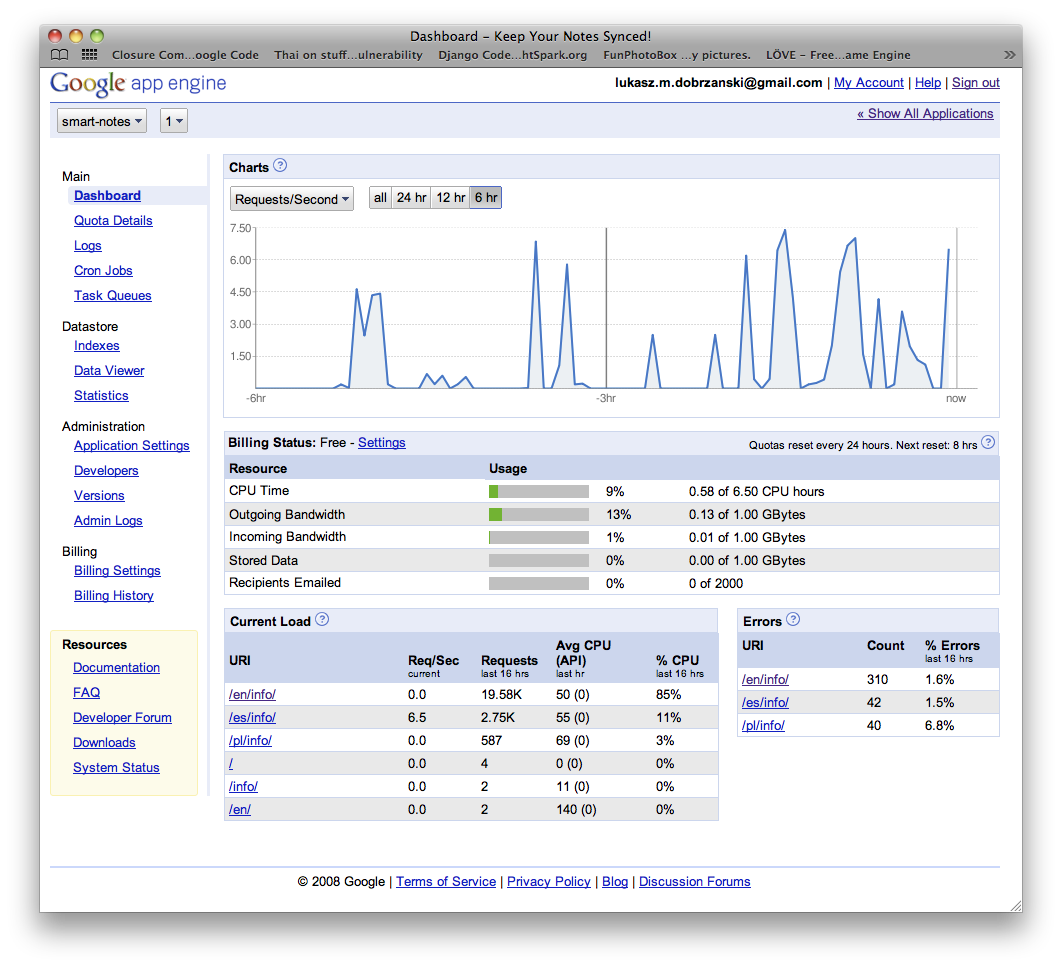
\includegraphics[scale=0.18]{img/DASH_Regular_stats.png}}
    \subfigure[\textbf{Application reaching the outgoing bandwidth limit on a heavy traffic situation with the maximum of 170 requests per second}.]{\label{fig:dash_out_of_bandwith}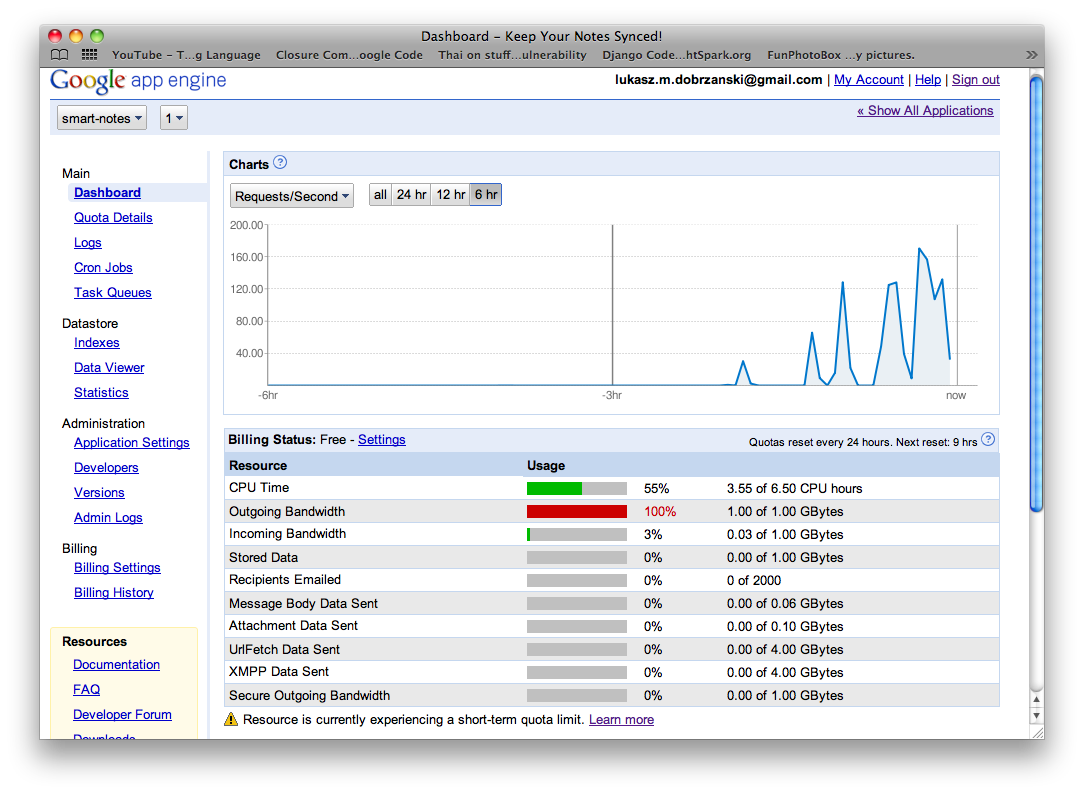
\includegraphics[scale=0.2]{img/DASH_Out_of_bandwith.png}}
  \end{center}
  \caption{The view on the public web-based SmartNotes interface with basic information regarding the project and authentication.}
  \label{fig:sn_dash_view}
\end{figure}
The system of quotas Google uses provides two-phase limitations: the daily limits and narrowed short time quotas, the latter providing protection for loading high peaks, before any malicious software or a testing one that disrespecting the resources could leave the target application out of resource in just a couple of minutes. The case of crossing quota was met during the tests by receiving responses with \texttt{503 Service Unavailable} status code when crossing the short time quota and \texttt{403 Forbidden} responses after running over the daily limits and was presented in Figure~\ref{fig:dash_out_of_bandwith}.
 
The author has chosen Open Source tools like \texttt{httperf} from HP and \texttt{autobench} wrapper to carry out tests for the main SmartNotes web page. These tools were chosen beyond researched others\footnote{That list includes tools like \texttt{siege}~\cite{siege_tool} and \texttt{ab}~\cite{ab_tool}, which are popular Open Source load testing programs.} due to support for a gradual increase of connection rate and an extended output. Each of the tests, whose results are presented in Figures~\ref{fig:sm_benchmark_normal}, \ref{fig:sm_benchmark_cache}, \ref{fig:sm_benchmark_static} and \ref{fig:sm_resp_time_comapre}, uses the same set of input parameters:
\begin{itemize}
              \item{500 connections per test. This connected with a 20-second connection timeout allowed to reach up to 400 concurrent connections.  }
              \item{3 requests per connection. This implies a total number of 1500 requests per test. The parameter was chosen with respect to the short term quota limit of $7, 400$ requests per minute.}
              \item{Generated connection rate was stored at 25 connections per second and by each test was gradually increased by the factor of 10 up to reaching the rate of 145 connections per second. That allowed to perform 12 tests for in each of test series.}
              \item{Each of tests is identified using multiplication of the generated connection rate and the number of requests per second as the horizontal axis labels. These values correspond to the theoretical request rate or the client-side request rate.}
\end{itemize}
 
The first technique tested here was a classical dynamic page using user language preferences in order to present internationalized content. For grater flexibility as well as minimizing the repetitions of common parts, the author decided to use template inheritance. Fundamentally, this lead to use template blocks in object-oriented programming. However, both of them cost the CPU time and in the case of a high-rated page they fail to be the most suitable solution. The most common approaches to this problem are presented in next two techniques: using caching or serving it as static content. One of parameters that has a great impact on the rest is the server-side connection rate that in Figures~\ref{fig:sm_benchmark_normal}, \ref{fig:sm_benchmark_cache} and \ref{fig:sm_benchmark_static} was presented using green lines. In the case of dynamic pages, the average connection rate becomes saturated when reaching the 45 connection per second, which gives the request rate of 135 requests per second.
\begin{figure}[ht]
  \begin{center}
              \includegraphics[scale=0.5]{charts/benchmarks/normal4X.pdf}
  \end{center}
  \caption{Response rate statistics for dynamic page served using the Django framework.}
              \label{fig:sm_benchmark_normal}
\end{figure}
This number is close to the abovementioned short time limit of $7, 400$ requests per minute. The test were done several times, narrowing the distance to this quota and watching for replies with the \texttt{200 OK} response code. Additionally, it is also interesting to observe the distribution of the minimum, average and maximum response rate with an increasing value of average request rate. In an ideal case, all of these four factors would follow an identical linear curve.    
 
The second technique is caching. It is a solution bundled into many web frameworks including Django, which - as noted in Section~\ref{sec:gae_general} - is supported by GAE. The concept of this technique is based on storing data in a fast, accessible space called cache and with the help of it repeating calls can shorten the request path. A simple usage of the caching system could look as presented in Listing~\ref{code:py_cache}. The function \texttt{get\_from\_cache} returns the data calculated by function called \texttt{some\_time\_consuming\_calculations} that consequently becomes located within control of \texttt{memcache}\footnote{Memcached is a distributed, memory based caching system. This is only one of possible caching backends such like file-cache or database storage engines. However, it is mostly used for its speed and support for multi-machine work mode.} for a time defined by the \texttt{expire\_time} variable. In case a subsequent calls come earlier than one hour from the first calculation of \texttt{data}, they will not call the \texttt{some\_time\_consuming\_calculations} function but will return the value stored by the \texttt{key} name.       
\lstset{language=Python,caption=Simple cache usage example in Python.,label=code:py_cache,
basicstyle=\scriptsize,         % the size of the fonts that are used for the code
showspaces=false,               % show spaces adding particular underscores
showstringspaces=false,         % underline spaces within strings
showtabs=false,                 % show tabs within strings adding particular underscores
tabsize=2,                    % sets default tabsize to 2 spaces
captionpos=b,                   % sets the caption-position to bottom
breaklines=true,                % sets automatic line breaking
breakatwhitespace=false,        % sets if automatic breaks should only happen at whitespace
escapeinside={\%*}{*)}          % if you want to add a comment within your code
}
\lstinputlisting{src/samples/py_cache.py}
When the \texttt{some\_time\_consuming\_calculations} is truly resource-consuming, this technique can bring efficient resource savings. The results from the plot in Figure~\ref{fig:sm_benchmark_cache} only slightly differ from the curves of the dynamic version from Figure~\ref{fig:sm_benchmark_normal}. HTTP headers shown in Listing~\ref{code:resp_headers} can help to avoid subsequent calls from a single user by using their browser-cache mechanisms. The test client was ignoring them as it was supposed to test the worst case scenario when all of the opened connections come from different users that browsers ignore the cache specific headers including \texttt{Expires}, \texttt{Vary}, \texttt{Last\-Modified}, \texttt{ETag} and \texttt{Cache\-Control}.
\lstset{language=HTML,caption=Server response headers for cached content.,label=code:resp_headers,
basicstyle=\scriptsize,         % the size of the fonts that are used for the code
showspaces=false,               % show spaces adding particular underscores
showstringspaces=false,         % underline spaces within strings
showtabs=false,                 % show tabs within strings adding particular underscores
tabsize=2,                    % sets default tabsize to 2 spaces
captionpos=b,                   % sets the caption-position to bottom
breaklines=true,                % sets automatic line breaking
breakatwhitespace=false,        % sets if automatic breaks should only happen at whitespace
escapeinside={\%*}{*)}          % if you want to add a comment within your code
}
\lstinputlisting{src/samples/headers_cache.txt}
 On the other hand, it does not mean that the use of caching did not bring any results. Because the requests to cache are much cheaper from the requests that involve the server-side operations, binding quota limits are lower and allow for $8,640,000$ API calls a day. The usage of \texttt{memcached} did help to reduce the CPU usage, which is a big advantage of this technique. However, it should be taken into account that usage of memory caching will consume additional memory, make the system slightly more complex and by itself is not a fault tolerant storage. Besides, one of the most serious problems regarding cache is the expiring content. In the case when a page component changes on certain pages, the easiest way to deal with the issue is to flush all the cache content. In the case of an application whose profile has a similar number of reads as writes, operations caches will be much harder to implement. Cache is a solution that suits best applications with a high read rate.     
\begin{figure}[ht]
  \begin{center}
              \includegraphics[scale=0.5]{charts/benchmarks/cache4X.pdf}
  \end{center}
  \caption{Response rate statistics for cached page. Realised using the Google memcache API.}
  \label{fig:sm_benchmark_cache}
\end{figure}
 
The last approach tested here was to serve the entire page as static content. It should be noted that the infrastructure used for this purpose differs strongly from the application server. It takes the advantage of storing stateless content and minimum server overhead. Implementation details belong to the Google company, however, there exist Open Source projects like \texttt{lighttpd}~\cite{lighthttp_tool} or \texttt{nginx}~\cite{nginx_tool} which share the same idea. Differences between them can be easy observed in Figure~\ref{fig:sm_benchmark_static}. Until reaching the level of 235 requests per second, the response rate curve was following the server-side request rate curve with a low variation, not crossing the factor of $5 \%$ of the average value. In this case, the CPU usage rate was even lower when using caching and did not require any additional memory usage like in the case of \texttt{memcached}. It should be noted that this technique requires much more work to be integrated with the application replacing its prior dynamic content, the task being sometimes even impossible to realize or resulting in bad user experience when completed in a wrong way. Thus, it is definitely an interesting option for applications that are stateless or use a significant number of various media files.            
 \begin{figure}[ht!]
  \begin{center}
              \includegraphics[scale=0.45]{charts/benchmarks/static4X.pdf}
  \end{center}
  \caption{Response rate statistics for static page with the use of static content server.}
\label{fig:sm_benchmark_static}
\end{figure}
\begin{figure}[ht!]
  \begin{center}
              \includegraphics[scale=0.45]{charts/benchmarks/final4X.pdf}
  \end{center}
  \caption{Comparison of average response times among various cases including serving dynamic content, caching response in memory and making use of static content server.}
              \label{fig:sm_resp_time_comapre}
\end{figure}

Comparison presented in Figure~\ref{fig:sm_resp_time_comapre} collates various techniques used together by focusing on the average response time. It is one of the parameters that has a huge impact on the final user experience. It clearly presents how much static content outperforms its concurrence. Second observation is that the case of the simple web page caching gave considerably low performance gain. Response rate curve for cached content started to reach higher values then the curve representing dynamic page response rate. Altogether caching brought measurable resource savings and become elastically integrated into SmartNotes application.  
